\documentclass{sig-alternate-2013}

\pdfminorversion=4
\pdfimageresolution=600

\usepackage{caption}
\usepackage{subfig}
\usepackage{todonotes}
\usepackage[hidelinks]{hyperref}
\usepackage{fixltx2e}
\usepackage{enumitem}
\usepackage[english]{babel}
\usepackage{microtype}

\clubpenalty=10000
\widowpenalty=10000

\makeatletter
\def\@copyrightspace{\relax}
\makeatother

\begin{document}

\hypersetup{pdftitle=Congestion-Aware Join Optimization in Key-Value Stores}
\hypersetup{pdfauthor={Xu Cui, Michael Mior, and Xinan Yan}}

\title{Congestion-Aware Join Optimization in Key-Value Stores}

\numberofauthors{3}
\author{
    \alignauthor{
        Xu Cui\\
        \affaddr{University of Waterloo}\\
        \email{xcui@uwaterloo.ca}
    }
    \alignauthor{
        Michael Mior\\
        \affaddr{University of Waterloo}\\
        \email{mmior@uwaterloo.ca}
    }
    \alignauthor{
        Xinan Yan\\
        \affaddr{University of Waterloo}\\
        \email{x29yan@uwaterloo.ca}
    }
}

\maketitle

\begin{abstract}
Applications which use key-value stores to execute higher-level queries need to aggregate data from multiple nodes.
In the case where all data is contained in main memory, the bottleneck becomes the network transfer of values from the datastore to the application.
When some keys become highly popular, network links to machines hosting these keys can become saturated and affect application performance.
In addition, nodes will compete with each other for bandwidth and uninformed traffic prioritization can result in reduced query execution time.
We demonstrate an approach based on software-defined networking (SDN) that takes advantage of replication and network performance measurements to effectively route requests over underutilized links.
\end{abstract}

\section{Introduction}

Recent trends have shown a proliferation of databases termed ``NoSQL'' which frequently eschew traditional database concepts such as referential integrity, ACID transactions, and high-level query languages for the sake of performance.
However, applications using these databases still have a need to perform complex queries.
Especially in the case of analytical queries, this may force the application designer to implement constructs such as joins at the application level.
This requires a significant amount of data transfer between nodes.
Given that it is common for data to be held in memory for performance reasons, the bottleneck for this data transfer is pushed up to the network layer.

\begin{figure}
    \centering
    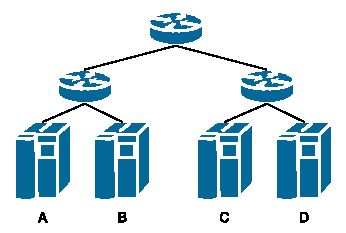
\includegraphics{figures/sample-topology.pdf}
    \caption{Sample network topology}\label{fig:sample-topology}
\end{figure}

Poor network scheduling can easily result in suboptimal query execution.
For example, consider the simple topology shown in Figure~\ref{fig:sample-topology}.
Assume a query is being processed that requires data to be sent between hosts A and C and hosts B and D that together will use the full capacity of all links in the network.
If the flows have equal bandwidth requirements, then fair bandwidth allocation will perform well.
However, if the flow between A and C requires twice the bandwidth of the flow between B and D, the first flow will have a longer completion time while it waits for available bandwidth.

In this scenario, if we schedule traffic using weighted fair queuing and reserve additional bandwidth for the first flow, it will complete sooner.
This results in a longer completion time for the second flow, but if we assume the query depends on all flows to be completed, we can see an overall reduction in query time.
Similarly, in the face of replicated data, a network-aware query processing engine can select routes and replicas to maximize link utilization and improve performance.
This type of intelligent network behaviour is difficult to configure in a traditional network stack.
With the advent of software-define networking (SDN), it is possible for a smart SDN controller to make global decisions based on the knowledge of higher-level application queries.
Furthermore, the controller can dynamically adapt the network to improve query processing efficiency.

As we discuss later, some existing query processing engines take into account network topology and link utilization when scheduling distributed queries.
However, there is relatively little work exploiting dynamic reconfiguration of the network to support query processing.
A centralized network controller which is aware of the dynamics of query processing is able to make smart routing decisions to optimize performance.
For example, flows for queries which are latency sensitive can be given priority over highly utilized links, while other flows can be routed to longer paths with lower utilization.
This can be done dynamically based on the state of the network.
Furthermore, the routing can be done using hardware switches as opposed to intelligent software routers, which minimizes latency and improves scalability.

In this work, we examine one possible application of SDN for improving the throughput of distributed join queries.
Specifically, we aim to schedule network traffic between servers processing distributed joins to optimize query completion time.
As identified above, improved scheduling can result in increased query performance.
We contribute a simple but effective method of flow scheduling in this use case.
We also identify several ways our work can be complemented with other techniques and extended to support alternative query models.

\section{System Overview}

\subsection{Query Model}

\begin{figure}
    \centering
    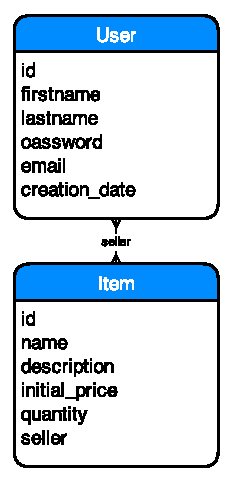
\includegraphics{figures/rubis-er.pdf}
    \caption{Simple query entities}\label{fig:entities}
\end{figure}

Our prototype system considers foreign key join queries between entity sets with a fixed join order and simple filtering on attributes of the first entity set.
For example, assume we have two entity sets \texttt{User} and \texttt{Item} with a one-to-many foreign key relating a user to each item as in Figure~\ref{fig:entities}.
A query (in SQL) syntax may look like \texttt{SELECT * FROM User, Item WHERE Item.User\_id = User.id AND Item.price > 20}.
In the future, we plan to consider a richer query language.
This will also present more interesting opportunities for optimization.

The execution model for these queries is very straightforward.
We consider the execution of the simple query given above.
We start by passing the query to each node which has entities of the class on the left side of the join (\texttt{Item}).
Those nodes will scan their local list of entities and apply the necessary filters (\texttt{price > 20}).
Each node then forwards the necessary foreign keys to nodes holding entities of the class on the right side of the join (\texttt{User}).
These nodes are then able to look up entities on the other side of the join and results can be passed back to the client.

\subsection{Architecture}

Our system uses OpenFlow~\cite{McKeown2008} enabled switches to allow centralized network control.
We currently pass all queries through our SDN controller which is running on the POX~\cite{Gude2008} platform.
Each host on the network contains a simple document store which is capable of answering requests both from client queries and other servers in the network.
When a query is received from a client, the server looks up entities on the left-hand side of the join in its local storage and requests the entities on the right side of the join from other servers in the network.
When a server receives a request from another server, it looks up the necessary entities to be joined locally and sends the reply back to the requesting server.
Once the server processing a client request receives responses from the other servers on the network, it can send a final response back to the client.

This results in the issue of stragglers we presented previously.
Note that the common technique of issuing a request multiple times to avoid stragglers is not helpful in our scenario.
As previously stated, our performance is bottlenecked by the available bandwidth.
Stragglers exist in our system because of a lack of available bandwidth as opposed to variations in node performance (which is what multiple issuance is designed to mitigate).
Furthermore, multiple issuance would place even stronger bandwidth pressure on our network, causing additional performance issues.
Instead, we mitigate the effect of stragglers by adjusting the bandwidth allocation for each flow.

\subsection{Flow Scheduling}

Simple approaches to bandwidth allocation such as max-min fairness pose significant problems in our settings.
If we were to use fair share allocation, then the node with the largest share of the query results, bottlenecked by available bandwidth, would become a straggler.
Nodes with a small share of query results could finish much more quickly only to wait for these stragglers.
To minimize the overall completion time of queries, we can allocate bandwidth to each node as the fraction of query results which will be returned by the node.
This will speed up stragglers at the expense of slowing down nodes with a smaller allocation.
However, the net result is a reduction in the average execution cost.

We currently deal with a read-only workload where the distribution of data is known by all nodes.
Each node is able to calculate the fraction of query results it will return.
A node can signal the expected fraction of the results for a query it will return by setting bits within the packet header.
When a new flow is issued for query processing, the controller can inspect these bits and assign an appropriate priority to each flow.
The controller is similar to a simple L2 learning switch.
However, we configure several queues for each switch port which allow us to provide bandwidth reservations to support variation in expected traffic volume.

We also change the flow table rules we install to match on the type of service (ToS) bits in the IP header.
Two of these eight bits are often used for explicit congestion notification (ECN).
We avoid these bits to allow ECN to operate uninhibited.
The remaining six bits are the differentiated services code point (DSCP) which are used to provide varying QoS guarantees for different flows.
We assume that the portion of the network our system is operating on is not carrying other traffic so we are free to set these bits as we choose.
To interconnect with other networks which may assign different meaning to these bits, we can simply zero these bits for any traffic passing through ingress/egress switches.

\section{Related Work}

The majority of work on query processing in key-value stores is in executing queries on data stored in distributed hash tables (DHTs) in peer-to-peer (P2P) networks.
For example, Harren et al.~\cite{Harren2002} propose a basic query model for executing complex queries in this scenario.
Their approach aims to minimize communication cost, but it is designed for P2P systems where the network is not under control of the application and is therefore unable to make use of network-aware techniques.
PIER~\cite{Huebsch2005} is a similar query processing engine over DHTs which is also not network-aware.
However, the query processing model used by PIER may be an interesting area to explore.

The traditional approach to optimizing network usage in distributed query processing is to apply smart key placement strategies to minimize the number of distributed transactions, and also the amount of data which must be transferred between nodes.
For example, Schism~\cite{Curino2010} uses graph partitioning techniques to reduce the cost of distributed transactions by up to 30\%.
Vila\c{c}a et al.~\cite{Vilaca2011} specifically target key-value stores and aim to improve locality in a multidimensional space of tags (such as foreign keys) applied to data items.
We expect partitioning techniques such as these to be complementary to our work.

There has also been some work in exploiting software-defined networking for big data applications.
Wang et al.~\cite{Wang2012} examined network traffic patterns in a Hadoop~\cite{Shvachko2010} cluster and identified opportunities to combine network-aware job scheduling with dynamic routing configuration to improve job completion time.
SmartJoin~\cite{Slagter2014} also examines network traffic patterns in Hadoop, specifically for join queries executed as MapReduce jobs.
SmartJoin attempts to balance the overhead of sending tuples to remote servers to be processed with the performance gains of parallel query processing.
These works hint at the benefits of network aware data processing systems, but focus on MapReduce jobs, while we we are interested in query processing over NoSQL database engines.

CloudTPS~\cite{Wei2012} provides a join query processing layer on top of NoSQL stores which enforces ACID semantics for transactions.
Our system does not currently consider transactional consistency, so this could be an interesting area to explore.
R\"{o}diger et al.~\cite{Rodiger2014} examine the affects of data locality with respect to distributed query processing.
Their Neo-Join algorithm is designed for efficient network usage by repartitioning data and scheduling network transfers to avoid cross-traffic.
These techniques exert no control over the network, which may provide further opportunities for optimization.

For example, Xiong et al.~\cite{Xiong2014} examine the usefulness of software-defined networking in supporting distributed analytical queries.
Their workload consists of read-only SQL queries where query processing is bandwidth-intensive.
They construct a global query optimizer which decides on join order and how query results should be passed between sites.
This work takes a similar approach to ours, but also identifies many opportunities for further work.

There are other advanced join operations which may benefit from software-defined
networking. Ntarmos et al.~\cite{Ntarmos2014} uses novel indexing techniques to
improve the performance of top-k joins for NoSQL databases which in turn
reduces both network latency and network traffics. This work did not explicit
use software-defined networking, however the amount of network traffic is one
important metric in their evaluation which hints possible network related
work in this domain.

\section{Evaluation}

We run all our experiments on a simulated network on a single machine using Mininet~\cite{Lantz2010}.
We use Open vSwitch~\cite{Pfaff2009} as our switch which supports queues with varying bandwidth guarantees.
Our controller uses the POX~\cite{Gude2008} platform and OpenFlow~\cite{McKeown2008} 1.0.

Queries use data taken from the RUBiS~\cite{Cecchet2002} benchmark, which is a Web application simulating an online auction.
We distribute data on users and the items they are selling between all nodes with no replication.

Each experiment is performed 5 times with the results are used to compute the data in the following sections.
The 95th percentile confidence interval is shown where appropriate.

\subsection{Micro Benchmark}
\begin{figure}
    \centering
    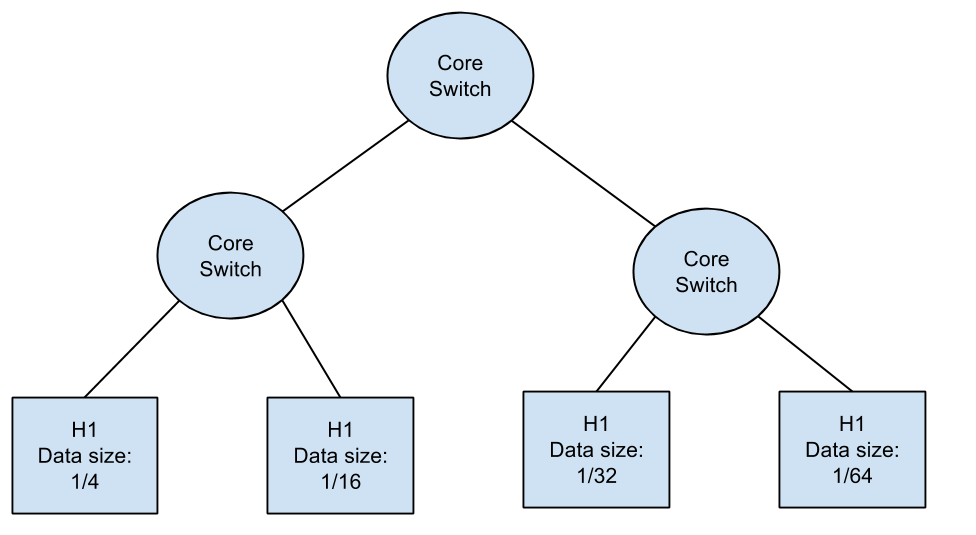
\includegraphics[scale=2.5]{figures/Join_micro_benchmark.png}
    \caption{Micro benchmark setup}\label{fig:micro_benchmark}
\end{figure}

First, we want to demonstrate the proof-of-concept of our design by evaluating our system with the simple topology shown in Figure~\ref{fig:micro_benchmark}.
We engineered the client query such that each server holds a different portion of the relevant data for the join operation.
That is, server 1 holds $1/4$ of the relevant item data and server 2, 3, and 4 hold $1/16$, $1/32$, $1/64$ of the relevant item data respectively.
The total sizes of the item and user data are approximately 9 MB and 2 MB\@.
In order to satisfy our assumption where the network is the bottleneck, we set the capacity of each link in the topology to 1 Mbps.
The client is connected directly to the core switch with a link of the same capacity.

In Figure~\ref{fig:micro_benchmark_total_time}, the red bars represent our system's baseline performance without our scheduling mechanism is turned off.
The average completion time without scheduling for each client query is over 180 seconds and also shows significant variation.
To provide predictable performance with our scheduling mechanism, we must first understand the characteristics of the costs for each component of the join operation.
In our case it is easy to predict the costs because we assigned different portions of relevant data to each server.
However, it is also easy in a real deployment scenario as the data distribution among servers is typically available or can be easily computed.
Recall that by design, server 1 is responsible for transmitting the largest flows between other servers and the client.
Therefore, our scheduling must take this information into consideration and ensure that server 1 has the largest minimum bandwidth guarantee for this particular operation.

Though we want server 1 to transfer its data as fast as possible, we do not want to starve other servers.
Therefore, we must also have reasonable minimum bandwidth guarantees for other servers.
Through experimentation, we found the most suitable minimum bandwidth guarantees on the 1 Mbps link for servers 2, 3, and 4 are 0.3 Mbps, 0.2 Mbps and 0.1 Mbps respectively.
We fixed these parameters and varied the minimum bandwidth guarantee for server 1 to study the network behaviour.
As shown by the right bars in Figure~\ref{fig:micro_benchmark_total_time}, there is a noticeable performance gain when we increase the minimum bandwidth guarantee of server 1 from 0.5 Mbps to 0.8 Mbps.
This shows that it is important to favour larger flows during a join operation to minimize the overall completion time.
We also want to highlight that we see diminishing returns as we further increase the guarantee.
This is caused by a significant increase in the completion time for other flows, hurting the overall performance.
In the best case, with 0.8 Mbps minimum bandwidth guarantee for server 1, the average completion time of the client query is 154 seconds which gives us almost 15\% performance gain over the baseline implementation.

\begin{figure}
    \centering
    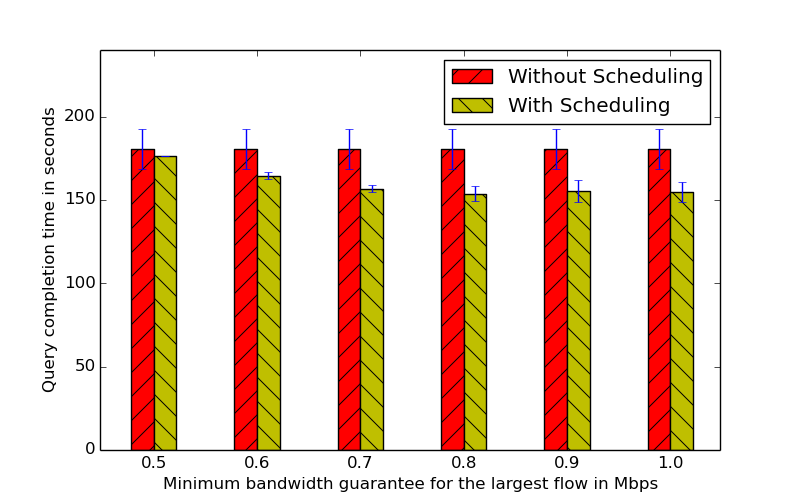
\includegraphics[scale=0.47]{figures/simple_topo_overall.png}
    \caption{Query completion time}\label{fig:micro_benchmark_total_time}
\end{figure}

Next, we further examine the performance results to understand why network scheduling helps.
Figure~\ref{fig:sub_query_completion_8} shows the subquery completion time for each server.
The per-server completion is calculated by the client after it fetches all the required data from each server.
The bars on the left are generated when traffic scheduling is disabled.
We see that server 1 takes the most time to complete and server 4 takes the least time.
This is expected due to the data distribution we defined above.
We can also see that when we enabled our network traffic scheduling mechanisms, the completion time for server 3 and server 4 slowed down slightly.
This is because most of the bandwidth will be allocated to help server 1 to finish its task as soon as possible.
However, The end result is that traffic scheduling reduces the average subquery completion time, which in turn reduces the overall query execution time.
We see that our experimental results match with our expectations.

\begin{figure}
    \centering
    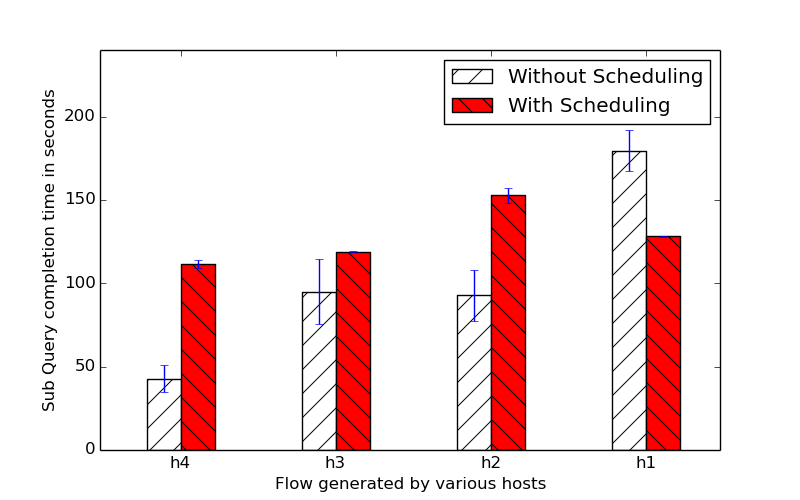
\includegraphics[scale=0.47]{figures/simple_topo_closer_8.png}
    \caption{Sub query completion time}\label{fig:sub_query_completion_8}
\end{figure}

\section{Future Work}

While our results are promising, we would like to take a more principled
approach to determine the theoretical gains possible for applying this
technique in order to clearly identify potential bottlenecks.  For example, we
have implemented a more realistic datacenter like topology with potentially
large number of servers. However, we find that our system requires a lot fine
tuning of minimum bandwidth guarantees for more complex systems. Theoretical
understanding of our system and approach could potentially enable us to
automate this fine-tuning process, which in turn allows us to perform a more
thorough evaluation on a larger scale with more realistic conditions. We feel
that there is potential to significantly improve the performance of our current
approach.  For example, we currently buffer all results at each server before
sending a reply.  Streaming results back to the client as they are received may
result in higher link utilization and increased efficiency.

There are many opportunities to combine this work with appropriate key
placement strategies for further performance optimizations.  For heterogeneous
networks, a key placement strategy which is network and workload aware may
provide significant performance advantages. On the flip side of data placement
problem is the data shipment problem where we can exploit our system's network
awareness to decide which node the data should be shipped to in order to
perform efficient join operation. Our current query execution model is very
simplistic and could be expanded to support richer queries and distributed
index data structures.  We would also like to investigate other query types
such as aggregation which we suspect would also benefit from our approach.
This presents new challenges in network scheduling, especially in the face of
concurrent queries of multiple different types.

Another promising direction is to consider the other kinds of network
topologies, such as fat tree topologies, where there exists multiple path
between any two hosts in the network. This enables our controller to use a
combination of network aware routing and minimum bandwidth guarantee techniques
to improve the overall performance of each query. We foresee that we will
evaluate our network-aware system against regular routing protocols such as
Open Shortest Path First routing to study the networking behaviours..

Our current system also does not deal with the possibility of updates or
replication.  There is potential to further exploit SDN techniques by allowing
low latency updates to data in the presence of the high bandwidth flows used
for query processing.  Replication provides further opportunity for
optimization as flows can be routed to multiple possible locations to avoid
bottleneck links or hosts.

We need to thoroughly study each of the aforementioned techniques to fully
understand their pros and cons in order to integrate all of them as a whole to
provide the optimal join operation for distributed NoSQL databases.

\section{Conclusion}

In this work, we examined opportunities to apply software-defined network
techniques to provide more efficient query processing over NoSQL databases.  We
demonstrated a simple technique using smart network scheduling to improve the
performance of distributed joins.  Our preliminary technique provides a
significant performance improvement over uninformed switching techniques.

We also presented several opportunities to further exploit of software-defined
network techniques to improve query processing.  As software-defined networking
becomes increasingly common in datacenters, we feel similar techniques will
become increasingly prevalent.  Little work has been done to exploit
software-defined networking in the context of NoSQL databases and distributed
data management.

\let\theOLDbibliography\thebibliography\renewcommand{\thebibliography}[1]{\theOLDbibliography{#1}%
\item[]\vspace*{0.5mm}}

\bibliographystyle{abbrv}
{\scriptsize
\bibliography{paper}
}

\end{document}
